%=====================================================================
\section{Complexity and memory analysis}\label{sec:complexity}
%=====================================================================

This section is analytic. It uses the specification's cost model ($L=1024$; 1 col = 2\,KB; $e=6r$ bytes, i.e.\ $2r$ lanes, of PSI traffic per changed absolute feature) and is not measured.
The PSI charge $e$ covers PSI's weight columns; PSI's own state pass (load and store of $P1,P2$, $12r=384$\,B per make) is not part of $e$ and is discussed in Section~\ref{sec:e2}.
Section~\ref{sec:experiments} measures the same quantities on real move sequences.

\begin{table}[htbp]
\centering\small
\caption{Per-move update cost, both perspectives (analytic). $\tau_c,\pi_c$: changed threat and pawn-pair features; $d_F=|S\symd C_{\text{new}}|$, $d_{\text{old}}=|S_{\text{prev}}\symd C_{\text{old}}|$; defaults $r=32$, $m=16$.}\label{tab:cost}
\begin{tabularx}{\linewidth}{@{}>{\raggedright}p{3.3cm}>{\raggedright}X>{\raggedright}X>{\raggedright\arraybackslash}p{2.7cm}@{}}
\toprule
Move type & NNUE (master) & VNNUE (default) & PSI extra (shared)\\
\midrule
Quiet non-king ($k=2$) & $2k+\sum_c(\tau_c+\pi_c)$ col & same & 128 lanes (384\,B)\\
Capture / e.p.\ / cap.-promo ($k=3$) & $2k+\sum_c(\tau_c+\pi_c)$ col & same & 192 lanes (576\,B)\\
Promotion ($k=2$) & $2k+\sum_c(\tau_c+\pi_c)$ col & same & 128 lanes\\
Own king, same block and half & $\min(|S|+\tau_{\text{full}},\,d_F,\,d_{\text{old}}+d_F+2\,\text{pass})$ + other side $k$ & min over the superset (adds $\mu r_K+k+\tau$ and ancestor) + other side $k$ & $k\cdot2r$ lanes\\
Own king across d/e, castling & $\min(|S|+\tau_{\text{full}},d_F)$ + other side & $\min(\dots,\text{finnyMirror if C6})$ + other side & $k\cdot2r$ lanes\\
Block change & refresh/Finny both sides & same (C3 superset) & $k\cdot2r$ lanes\\
$t$-ply lazy catch-up & $\sum_jk_j$ col + about $t$ passes & $|\supp\sum_j\delta_j|$ col + 1 pass & $\sum_jk_j\cdot2r$ lanes (eager)\\
\midrule
Per evaluation & pairwise 1024 products; fc\_0 $\le32{,}768$ MACs & same & $2\cdot512+1024=2048$ MACs\\
Per evaluation, C2$'$ & -- & $+\,r_KL$ MACs per perspective (32,768 for both at $r_K=16$) & \\
\bottomrule
\end{tabularx}
\end{table}

Table~\ref{tab:cost} gives the per-move costs.
Two statements are proved.
First, per build event, from identical accumulator and cache state and under a shared cost function (the T24 assumptions), VNNUE's FT column cost is $\le$ the minimum over Stockfish's candidates.
This does not compose over a search: see E3 (Section~\ref{sec:e3}), where greedy C4 raises whole-trace columns by 20.3\% on lazy trees.
Second, PSI's weight-column traffic is at most $e/(4L)=4.6875\%$ of NNUE's PSQ column traffic whenever NNUE streams at least $k$ columns per perspective (T25).
The bound is tight for quiet moves.
The ratio falls once NNUE's passes and threat churn (``3--4$\times$ as many changing threat features as piece features in a typical midgame''~\cite{nnuepytorchdocs}) are included, but such ratios must also charge PSI its state pass.
Non-king moves therefore do strictly \emph{more} work in VNNUE.
King moves are never worse in column count per event, under the T24 cost assumptions.
Wall-clock effects depend on cache residency: the 24\,KB $V$ table, plus 48\,KB if $V^{\circ2}$ is stored, should stay in L1/L2, whereas FT columns stream from L3 or DRAM.
We have not measured this.

The per-evaluation PSI readout costs 2048 multiply-adds at $r=32$, $m=16$.
That is 6.3\% of a dense fc\_0, and a larger share of Stockfish's sparse fc\_0.
The factored C2$'$ mode costs $r_KL$ MACs per perspective per evaluation.
At $r_K=16$ this is 16,384 MACs per perspective, i.e.\ 32,768 for both perspectives, equal to a dense fc\_0 ($1024\times32$): a real tax that has to be bought back by memory savings.

\begin{table}[htbp]
\centering\small
\caption{Memory (analytic). $|P|$: number of king regions in C2$'$. Units: MB $=10^6$\,B, KB $=1024$\,B.}\label{tab:memory}
\begin{tabularx}{\linewidth}{@{}>{\raggedright}p{3.0cm}>{\raggedright}p{2.6cm}>{\raggedright}p{2.2cm}>{\raggedright}X>{\raggedright\arraybackslash}X@{}}
\toprule
Item & NNUE master & VNNUE default & + C2 merged ($r_K=16$) & + C2$'$ factored ($|P|=4$, $r_K=16$)\\
\midrule
PSQ FT table & $67{,}584\times1024\times2$\,B $=138.4$\,MB & 138.4\,MB & 138.4\,MB + $U$: 3.1\,MB + $V_K$: 11\,KB & $3\cdot4\cdot704\cdot1024\cdot2$\,B $=17.3$\,MB + 3.1\,MB $=20.4$\,MB\\
PSI $V$ / $V^{\circ2}$ & -- & 24\,KB / 48\,KB & same & same\\
$\Lambda$, $b^z$ & -- & 512\,B + 64\,B & same & same\\
fc\_0 extra & -- & 32\,KB & same & same\\
Per-ply state & $2\times2$\,KB + threat state & + 64\,B ($P1$) + 128\,B ($P2$), once per position & + $2\times32$\,B ($y$) & same\\
Finny entry & acc + board & unchanged & + $y$ (32\,B) & + $y$\\
\bottomrule
\end{tabularx}
\end{table}

Table~\ref{tab:memory} gives the memory footprint.
The only large potential saving is C2$'$, which would make the PSQ table about 6.8 times smaller.
It pays the readout tax above, and E5 (Section~\ref{sec:e5}) shows that the integer-factor constraint is costly without quantization-aware training.

%=====================================================================
\section{Experiments}\label{sec:experiments}
%=====================================================================

\paragraph{Setup and scope.}
All numbers in this section are copied from \texttt{experiments/RESULTS.md}, which is generated mechanically from \texttt{experiments/results/*.json}.
The machine was a 4-core Windows laptop CPU with Python 3.14, numpy 2.4, torch 2.10 (CPU) and python-chess 1.11, and all seeds were fixed.
This is a Python prototype.
Op and byte counts are exact counts under an explicit cost model.
Wall-clock numbers are numpy/torch proxies that do not represent SIMD C++.
The search traces come from a toy alpha-beta searcher, not from Stockfish.
\textbf{No statement in this section concerns playing strength, Elo or nps.}

\paragraph{Pre-registered hypotheses.}
The design specification stated three hypotheses before the experiments, which are our own priors:
H1, PSI byte overhead $\le4.7\%$ of PSQ column traffic (the T25 bound) under the byte model;
H2, at $r_K=16$ with $\Delta U$ formed on the fly, the low-rank (``Woodbury'') source wins fewer than 10\% of own-king events;
H3, C4's column saving from cancellation is $<1\%$.

\paragraph{Data.}
We used three sources (Table~\ref{tab:data}).
The first is the first 3,000 standard games from the January 2013 Lichess database~\cite{lichessdb} (CC0), giving 202,984 positions.
The second is 30 self-play games of a depth-2 alpha-beta with quiescence (2,440 positions).
The third is search traces from 200 roots (160 from Lichess games, 40 from self-play), searched by alpha-beta at depth 3 with capture quiescence (at most 4 plies) and MVV-LVA ordering.
Each tree was capped at 2,500 nodes, and 116 trees hit the cap.
The traces contain 389,664 make events, stored as DFS pre-order node lists, i.e.\ exactly the make/unmake stream of an accumulator stack.
\emph{Eager} evaluation evaluates every node.
\emph{Lazy} evaluation evaluates the roots, all quiescence and leaf nodes, and interior nodes with probability 0.3.
The feature model is a simplified K32H3: 32 mirrored own-king buckets, the 3 verified blocks, and 704 local features (67,584 per perspective).
Threat and pawn-pair columns, PSQT outputs and layer stacks are \emph{not} modelled inside the accumulator.
A threat \emph{proxy} is counted for byte accounting only.

\begin{table}[htbp]
\centering\small
\caption{Data used by the experiments.}\label{tab:data}
\begin{tabularx}{\linewidth}{@{}>{\raggedright}p{3.6cm}>{\raggedright}X>{\raggedright\arraybackslash}p{3.8cm}@{}}
\toprule
Source & Content & Size\\
\midrule
Lichess 2013-01, first 3,000 standard games & real human move sequences and results & 202,984 positions; 175,984 training positions (ply $\ge8$)\\
Self-play & depth-2 alpha-beta + quiescence, material+PST eval, 30 games & 2,440 positions\\
Search traces & 200 roots, depth 3 + capture quiescence, 2,500-node cap (116 trees hit it) & 389,664 make events\\
\bottomrule
\end{tabularx}
\end{table}

\subsection{E1: exactness}\label{sec:e1}

The prototype uses $L=64$ int16 lanes, PSI with $r=32$ and $m=16$, and C2 rank $r_K=8$.
E1 runs on subsets: the first 300 Lichess games (19,559 positions), all self-play games (2,440), and 15 (eager) / 40 (lazy) of the 200 search roots (34,534 / 88,026 nodes).
This is why its build counts (e.g.\ 39,118 on Lichess) are smaller than those of E3 (405,968).
The K32H3 table is the \emph{materialized merged} C2 table $W[\mathrm{blk},\kappa]=W^0[\mathrm{blk}]+U[\mathrm{blk},\kappa]V_K$, computed modulo $2^{16}$, so the Woodbury identity is tested on the same table every other source uses.
At every accumulator build, every available source is computed with numpy int16 wrapping adds and compared bit for bit with the from-scratch refresh.
The sources are refresh, Finny, hybrid, SF chain catch-up with two-ply cancellation, VNNUE ancestor net-delta, and the Woodbury transition.
The chosen source's value is reused downstream, so errors would propagate.
PSI checks run at every make event.
We tested two weight regimes: \emph{normal} weights, and \emph{stress} weights ($|W^0|\le6000$, $|U|\le300$, $|V_K|\le127$, $|b|\le20000$), under which partial sums regularly leave the int16 range.
Under stress weights most \emph{final} lane values are themselves out of int16 range (e.g.\ 1,762,588 of 2,503,552 lane finals on Lichess); for these lanes bit-exactness means agreement modulo $2^{16}$ with the refresh, not a correct int16 decode.

\begin{table}[htbp]
\centering\small
\caption{E1 totals (all runs, both weight regimes).}\label{tab:e1}
\begin{tabular}{@{}lr@{}}
\toprule
Total & Value\\
\midrule
accumulator candidate checks (source value $=$ refresh, bit-exact) & 6,670,640\\
mismatches & \textbf{0}\\
builds where a lane decoded wrongly although the exact final value was in int16 range & \textbf{0}\\
(candidate, lane) results with a partial sum outside int16 but in-range final value, all exact & 58,084,584\\
PSI / $y$ / feature-delta checks & 7,803,876\\
PSI / $y$ / feature-delta mismatches & \textbf{0}\\
\bottomrule
\end{tabular}
\end{table}

\begin{table}[htbp]
\centering\small
\caption{E1 per run (checks are identical for normal and stress weights; the last column is from the stress runs). ``VN $\mu=0$'' makes Woodbury artificially cheap so that its outputs are reused often.}\label{tab:e1runs}
\begin{tabular}{@{}lllrrr@{}}
\toprule
dataset & eval & policy & builds & \hd{checks\\(0 mismatches)} & \hd{exact despite out-of-\\range partial sums}\\
\midrule
games\_lichess & eager & SF $\mu=1$ & 39,118 & 153,205 & 2,824,741\\
games\_lichess & eager & VN $\mu=1$ & 39,118 & 155,658 & 2,754,658\\
games\_lichess & eager & VN $\mu=0$ & 39,118 & 155,658 & 2,681,726\\
games\_selfplay & eager & SF $\mu=1$ & 4,880 & 19,066 & 364,975\\
games\_selfplay & eager & VN $\mu=1$ & 4,880 & 19,468 & 358,846\\
games\_selfplay & eager & VN $\mu=0$ & 4,880 & 19,468 & 344,355\\
trees & eager & SF $\mu=1$ & 69,068 & 273,612 & 4,878,069\\
trees & eager & VN $\mu=1$ & 69,068 & 275,609 & 4,776,872\\
trees & eager & VN $\mu=0$ & 69,068 & 275,609 & 4,734,806\\
trees & lazy & SF $\mu=1$ & 168,696 & 656,071 & 11,569,113\\
trees & lazy & VN $\mu=1$ & 168,696 & 665,948 & 11,467,537\\
trees & lazy & VN $\mu=0$ & 168,696 & 665,948 & 11,328,886\\
\bottomrule
\end{tabular}
\end{table}

\paragraph{Results.}
Tables~\ref{tab:e1} and~\ref{tab:e1runs} show the results.
There were 6,670,640 accumulator-source checks and 7,803,876 PSI, $y$-state and feature-delta checks, all with 0 mismatches.
The PSI checks cover the following:
\begin{itemize}[leftmargin=*,itemsep=1pt]
\item incremental $P1,P2$ against full recomputation;
\item $P1^2-P2$ is always even;
\item incrementally maintained $E$ (T14);
\item the multi-head readout against a brute-force sum over all present piece pairs (T13);
\item the Black view as a lane permutation under tying (T21).
\end{itemize}
In 58,084,584 (candidate, lane) results the update path left the int16 range and still decoded exactly, as T7(c) predicts.
In the lazy VN runs with $\mu=1$ (resp.\ $\mu=0$), 36,864 (resp.\ 37,128) builds used the ancestor net-delta and 3,081 (resp.\ 9,955) used Woodbury.

\paragraph{Saturation (T8), empirically.}
Along the first 200 Lichess games, each perspective's accumulator was updated incrementally with wrapping adds and with saturating adds, and each was compared with the same arithmetic applied from scratch.
With normal weights nothing saturated: 0 mismatches of 25,680 for both.
With stress weights, 25,280 of 25,680 saturating accumulators differed (1,518,777 lanes).
In 456,904 of those lanes the exact final value was in range, so saturation gave a wrong answer that wrapping got right.
Wrapping had 0 mismatches.

\subsection{E2: PSI overhead}\label{sec:e2}

The cost model is $L=1024$; 1 col = 2048\,B; 1 pass = 4096\,B; PSI = 192\,B and 64 lanes per changed absolute feature, applied eagerly at every make event; threat-proxy columns are 1\,KB.
The PSI charge covers its weight columns only.
NNUE is charged its accumulator passes, but PSI is \emph{not} charged its own state pass (load and store of $P1,P2$: $2\cdot(64+128)=384$\,B per make).
The ``incl.\ passes'' ratios below are therefore asymmetric and favour PSI: counting the state pass, a quiet move costs PSI $384+384=768$\,B against NNUE's 16,384\,B, i.e.\ the same 4.69\% as the column-only ratio rather than 2.34\%.

\begin{table}[htbp]
\centering\small
\caption{Move statistics. $k_a$: changed absolute features per move; $|S|$: active PSQ features.}\label{tab:movestats}
\begin{tabular}{@{}lrrrrrrr@{}}
\toprule
dataset & positions & quiet & capture & \hd{king\\quiet} & castling & \hd{$k_a$\\mean} & \hd{$|S|$ mean\\/ p50 / p95}\\
\midrule
games\_lichess & 202,984 & 64.5\% & 22.1\% & 9.7\% & 2.3\% & 2.279 & 23.048 / 25 / 32\\
games\_selfplay & 2,440 & 60.9\% & 21.4\% & 15.6\% & 0.0\% & 2.229 & 21.48 / 22 / 32\\
trees & 389,664 & 43.2\% & 48.8\% & 4.9\% & 0.1\% & 2.518 & 23.793 / 25 / 31\\
\bottomrule
\end{tabular}
\end{table}

\begin{table}[htbp]
\centering\small
\caption{Per move type, Lichess games (eager), from the main E2--E4 run, whose Finny cache persists across games (stale entries; see Section~\ref{sec:e3}). The SF and VN column counts on king moves, promotions and captures therefore reflect our simulator's cache model and are not evidence that VNNUE saves bytes there; Table~\ref{tab:reset} gives the cache-reset values. Columns and bytes per move, both perspectives, means. Overhead ratios are totals over the class; PSI is charged weight columns only, not its state pass.}\label{tab:e2}
\begin{tabular}{@{}lrrrrrrr@{}}
\toprule
move type & count & \hd{SF\\cols} & \hd{VN\\cols} & \hd{SF\\bytes} & \hd{PSI\\bytes} & \hd{PSI/PSQ\\col.\ bytes} & \hd{incl.\\passes}\\
\midrule
quiet & 128,999 & 4 & 4 & 16,384 & 384 & 4.69\% & 2.34\%\\
capture & 44,132 & 7.724 & 7.241 & 24,010 & 576 & 3.64\% & 2.40\%\\
king\_quiet & 19,305 & 25.332 & 14.822 & 63,173 & 384 & 0.74\% & 0.61\%\\
castling & 4,519 & 33.317 & 28.883 & 76,425 & 768 & 1.13\% & 1.00\%\\
king\_capture & 2,407 & 27.734 & 17.363 & 67,551 & 576 & 1.01\% & 0.85\%\\
promotion & 502 & 20.45 & 10.765 & 50,074 & 384 & 0.92\% & 0.77\%\\
en\_passant & 90 & 6 & 6 & 20,480 & 576 & 4.69\% & 2.81\%\\
capture\_promotion & 30 & 17.133 & 11.933 & 43,281 & 576 & 1.64\% & 1.33\%\\
\bottomrule
\end{tabular}
\end{table}

\begin{figure}[htbp]
\centering
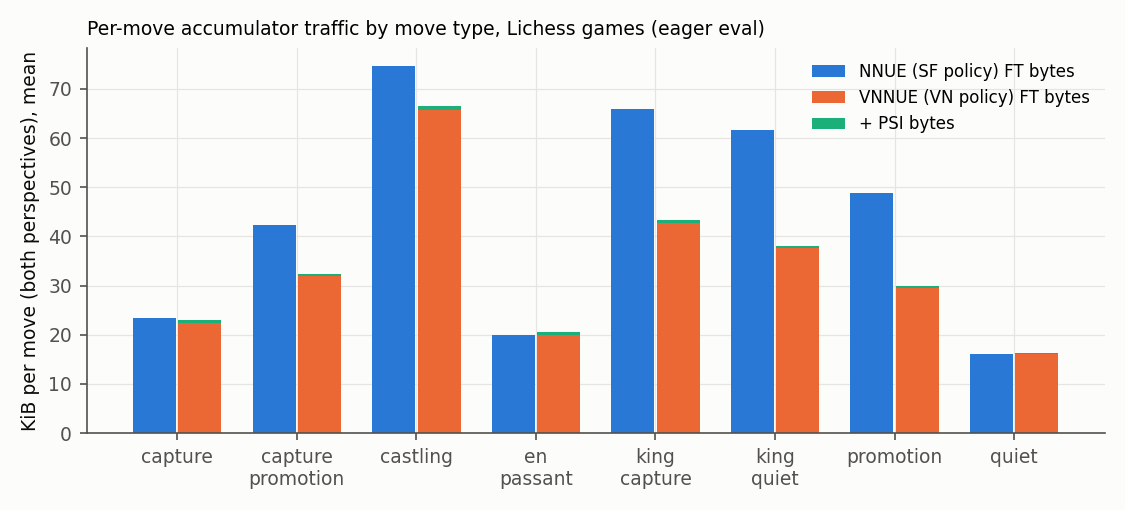
\includegraphics[width=0.85\linewidth]{figures/e2_bytes_per_move_type.png}
\caption{E2: per-move FT bytes, NNUE vs VNNUE, plus PSI bytes, by move type (Lichess games, eager; main run with a persisting Finny cache, so the king-move differences reflect our simulator, see Table~\ref{tab:reset}).}\label{fig:e2}
\end{figure}

\paragraph{Results.}
Tables~\ref{tab:movestats}--\ref{tab:e2} and Figure~\ref{fig:e2} show the results.
On a quiet move PSI adds exactly 4.69\% of PSQ column bytes, which is the T25 bound; the bound is tight at $k=2$.
Over all Lichess moves PSI adds 2.68\% of PSQ column bytes.
This drops to 1.75\% once NNUE's accumulator passes are counted (but not PSI's state pass, see above), and to 1.14\% once the threat proxy is counted (self-play: 2.62\%, 1.71\%, 1.19\%); the threat-proxy figures are computed on the first 600 Lichess games (36,701 moves).
On that subset the threat proxy changes 6.798 features per move and perspective on average, 2.98 times the number of changed piece-square features, slightly below the ``3--4$\times$ in a typical midgame'' stated in the nnue-pytorch documentation~\cite{nnuepytorchdocs}.
Own-king moves (quiet, captures and castling) are 13.1\% of Lichess moves (26,231 of 199,984).
In games, 8.94\% of accumulator builds need a table change (king bucket, mirror or block).
Hypothesis H1 (PSI overhead $\le4.7\%$ of PSQ column bytes) therefore holds under the byte model, which charges PSI for weight columns only.
Whether the extra bytes cost wall-clock time in an engine is not measured.

\subsection{E3: source selection and net-delta catch-up}\label{sec:e3}

We compare four policies, each simulated independently over the whole event stream with its own Finny caches and materialized accumulators:
\begin{itemize}[leftmargin=*,itemsep=1pt]
\item \textbf{SF}, a Stockfish-like rule: chain catch-up if there is no table change, otherwise hybrid if its conditions hold, otherwise Finny;
\item \textbf{SFmin}: chain catch-up whenever available (as SF), otherwise the argmin over \{refresh, Finny, hybrid\}; the SF-set minimum in Table~\ref{tab:e3cf} is defined the same way;
\item \textbf{VN\_noC4}, the argmin over \{refresh, Finny, hybrid, chain\}, i.e.\ SFmin except that it may skip an available chain;
\item \textbf{VN}, which is VN\_noC4 plus ancestor net-delta (C4).
\end{itemize}
The argmin scalar is $\mathrm{cols}+\mu\cdot\mathrm{mcols}+2\cdot\mathrm{passes}$.
Woodbury is not in these candidate sets; it is evaluated separately in E4.
\emph{Cache model.} In the main run (Tables~\ref{tab:e3}--\ref{tab:hybrid}) each policy keeps one Finny cache for the whole dataset, so entries persist across games and search trees and are updated only when a Finny, refresh or hybrid source is used.
They are therefore \emph{stale}, not cold: an entry may come from an unrelated game.
Stockfish clears its refresh table on \texttt{ucinewgame} and its cache is warmed by the search itself.
We therefore reran all four policies with the cache cleared at every root (each game and each search tree, warmed by the run itself; Table~\ref{tab:reset}).


\begin{table}[htbp]
\centering\small
\caption{E3 whole-trace totals per policy (stateful simulation).}\label{tab:e3}
\begin{tabular}{@{}llrrrrrr@{}}
\toprule
dataset & policy & \hd{cols/\\eval} & \hd{passes/\\eval} & \hd{FT bytes/\\eval} & \hd{cols\\vs SF} & \hd{passes\\vs SF} & \hd{PSI/FT\\bytes}\\
\midrule
games\_lichess/eager & SF & 7.841 & 2.079 & 24,576 & 1.0000 & 1.0000 & 1.75\%\\
 & SFmin & 6.438 & 2 & 21,377 & 0.8211 & 0.9618 & 2.02\%\\
 & VN\_noC4 & 6.436 & 2 & 21,373 & 0.8208 & 0.9618 & 2.02\%\\
 & VN & 6.436 & 2 & 21,373 & 0.8208 & 0.9618 & 2.02\%\\
\midrule
games\_selfplay/eager & SF & 7.877 & 2.102 & 24,744 & 1.0000 & 1.0000 & 1.71\%\\
 & SFmin & 6.382 & 2 & 21,263 & 0.8102 & 0.9513 & 1.99\%\\
 & VN\_noC4 & 6.38 & 2 & 21,257 & 0.8099 & 0.9513 & 1.99\%\\
 & VN & 6.379 & 2 & 21,256 & 0.8098 & 0.9513 & 1.99\%\\
\midrule
trees/eager & SF & 5.586 & 2.088 & 19,990 & 1.0000 & 1.0000 & 2.42\%\\
 & SFmin & 5.399 & 2 & 19,249 & 0.9666 & 0.9580 & 2.51\%\\
 & VN\_noC4 & 5.394 & 2 & 19,239 & 0.9656 & 0.9580 & 2.51\%\\
 & VN & 5.398 & 2 & 19,248 & 0.9665 & 0.9580 & 2.51\%\\
\midrule
trees/lazy & SF & 5.842 & 2.129 & 20,683 & 1.0000 & 1.0000 & 2.44\%\\
 & SFmin & 5.665 & 2.056 & 20,022 & 0.9697 & 0.9657 & 2.52\%\\
 & VN\_noC4 & 5.805 & 2.036 & 20,228 & 0.9938 & 0.9564 & 2.49\%\\
 & VN & 7.026 & 2 & 22,581 & 1.2027 & 0.9396 & 2.23\%\\
\bottomrule
\end{tabular}
\end{table}

\begin{table}[htbp]
\centering\small
\caption{Per-event counterfactual (T24 sanity check): at every build event, min over the full VN set $\le$ min over SF's set.}\label{tab:e3cf}
\begin{tabular}{@{}llcrr@{}}
\toprule
dataset & policy & \hd{holds at\\every event} & \hd{summed saving\\(col-equiv.)} & \hd{fraction of\\SF-set cost}\\
\midrule
games\_lichess/eager & VN\_noC4 & True & 347 & 0.02\%\\
games\_lichess/eager & VN & True & 534 & 0.03\%\\
games\_selfplay/eager & VN\_noC4 & True & 7 & 0.03\%\\
games\_selfplay/eager & VN & True & 9 & 0.04\%\\
trees/eager & VN\_noC4 & True & 3,335 & 0.09\%\\
trees/eager & VN & True & 3,760 & 0.10\%\\
trees/lazy & VN\_noC4 & True & 407,985 & 9.96\%\\
trees/lazy & VN & True & 948,711 & 18.73\%\\
\bottomrule
\end{tabular}
\end{table}

\begin{figure}[htbp]
\centering
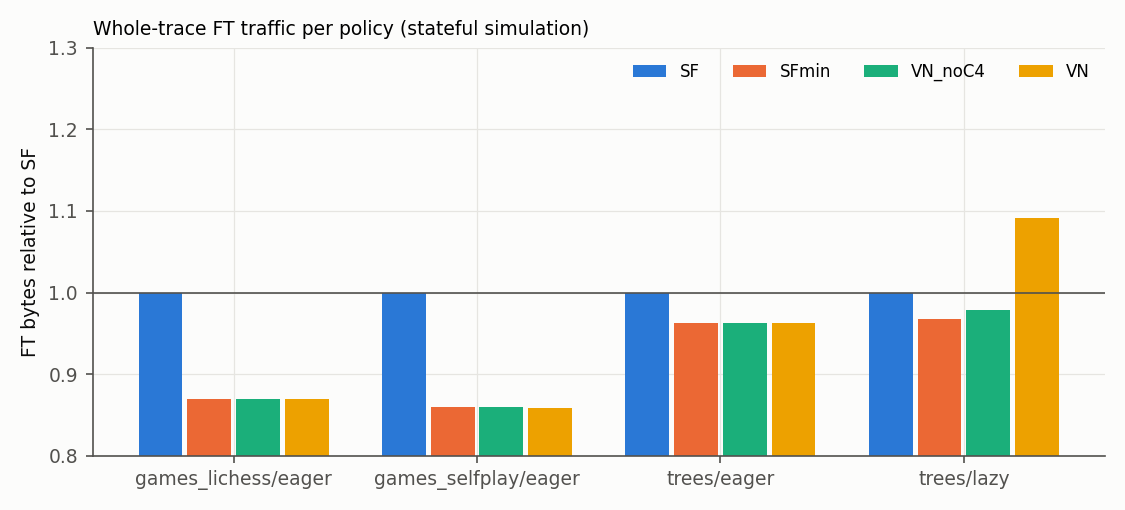
\includegraphics[width=0.8\linewidth]{figures/e3_policy_totals.png}
\caption{E3: whole-trace FT bytes per policy, relative to SF (main run, in which the Finny cache persists across games and trees; the SF/SFmin gap shrinks with a per-root reset, Table~\ref{tab:reset}).}\label{fig:e3}
\end{figure}

\paragraph{Results.}
Tables~\ref{tab:e3}--\ref{tab:e3cf} and Figure~\ref{fig:e3} show the results.
\begin{enumerate}[leftmargin=*,itemsep=2pt]
\item \emph{The never-worse property holds per event}, as T24 guarantees.
\item \emph{The superset adds almost nothing.}
In the eager runs, almost all of the gain of VN over the SF \emph{rule} comes from taking the argmin over SF's \emph{own} set (SFmin); on lazy trees VN is worse than SF (item~3).
SFmin and VN cost within 0.1\% of each other in the eager runs.
The per-event savings of VN over the SF-set minimum (at most 0.10\% in eager runs, Table~\ref{tab:e3cf}) come from VN being allowed to pick refresh, Finny or hybrid where SFmin is forced to chain, plus the ancestor candidate; Woodbury is not in these sets.
\item \emph{The size of the SFmin gain is a simulator artifact.}
In the main run the Finny cache persists across games and trees, so its entries are stale, and SF's hybrid rule is often more expensive than a plain Finny refresh: at table changes on Lichess games, hybrid averages 36.7 columns and Finny 16.3 (Table~\ref{tab:hybrid}).
With the cache cleared at every root (Table~\ref{tab:reset}), the column ratio of SFmin to SF on Lichess games rises from 0.8211 to 0.9387 (FT bytes 0.9466), and to 0.9780 on eager trees.
What remains comes from our model of the SF rule, which never chooses a plain refresh; with a reset cache, hybrid still averages 30.4 columns at table changes on Lichess games against 18.8 for Finny.
This is \textbf{not} evidence about Stockfish itself, whose hybrid conditions and cache warm-up we model only approximately, and it is no evidence that VNNUE saves bytes on king moves.
\item \emph{Greedy C4 hurts in a stateful search.}
On the lazy trees, VN uses 20.3\% more columns and 9.2\% more FT bytes per evaluation than SF, with 6\% fewer passes (with the cache reset per root: 1.2169 and 1.0992).
The cause is that C4 skips materializing intermediate accumulators that sibling nodes would later reuse.
The per-event counterfactual ``saving'' (18.73\%) is therefore misleading: the policies diverge in state, and per-event optimality does not compose.
Even without C4, VN\_noC4 is worse than SFmin on lazy trees (5.805 vs 5.665 cols/eval, 20,228 vs 20,022 FT bytes/eval) despite a 9.96\% per-event counterfactual saving, so the non-composition is a property of greedy argmin over the larger set, not only of C4.
\item \emph{Cancellation is larger than our prior.}
Within catch-ups of length $\ge2$ (227,886 events in the lazy run), cancellation saved 10.85\% of columns, with mean net-support ratio 0.905.
Stockfish's PR~\cite{sfpr5988} gives no figure for how much cancellation saves; its author estimated informally that about 0.2\% of three-move updates have one side moving the same piece twice, which is a different statistic from our column saving.
We attribute our higher saving to frequent same-square quiescence recaptures in our toy trees.
Our own prior H3 (column saving $<1\%$) is therefore not supported, but the whole-trace effect of greedy C4 is negative.
\end{enumerate}
A caveat: our ``lazy'' mode removed only 4\% of evaluations, because most nodes in these trees are quiescence nodes.

\begin{table}[htbp]
\centering\small
\caption{E3 rerun with the Finny cache cleared at every root (each game, each search tree), warmed by the run itself (\texttt{e3\_cache\_reset.py}; RESULTS.md \S2.7). Ratios are relative to SF in this rerun.}\label{tab:reset}
\begin{tabular}{@{}llrrrrr@{}}
\toprule
dataset & policy & \hd{cols/\\eval} & \hd{FT bytes/\\eval} & \hd{cols\\vs SF} & \hd{FT bytes\\vs SF} & \hd{per-event saving\\vs SF-set min}\\
\midrule
games\_lichess/eager & SF & 7.939 & 24,777 & 1.0000 & 1.0000 & \\
 & SFmin & 7.452 & 23,455 & 0.9387 & 0.9466 & \\
 & VN & 7.45 & 23,450 & 0.9384 & 0.9464 & 0.02\%\\
\midrule
games\_selfplay/eager & SF & 7.682 & 24,344 & 1.0000 & 1.0000 & \\
 & SFmin & 7.094 & 22,720 & 0.9234 & 0.9333 & \\
 & VN & 7.09 & 22,713 & 0.9230 & 0.9330 & 0.03\%\\
\midrule
trees/eager & SF & 5.527 & 19,870 & 1.0000 & 1.0000 & \\
 & SFmin & 5.405 & 19,262 & 0.9780 & 0.9694 & \\
 & VN & 5.406 & 19,263 & 0.9781 & 0.9695 & 0.11\%\\
\midrule
trees/lazy & SF & 5.78 & 20,555 & 1.0000 & 1.0000 & \\
 & SFmin & 5.671 & 20,034 & 0.9812 & 0.9746 & \\
 & VN\_noC4 & 5.811 & 20,240 & 1.0055 & 0.9847 & 9.96\%\\
 & VN & 7.033 & 22,595 & 1.2169 & 1.0992 & 18.72\%\\
\bottomrule
\end{tabular}
\par\smallskip
\begin{tabular}{@{}lrrrr@{}}
\toprule
Lichess games, per move & \hd{SF cols\\(main run)} & \hd{VN cols\\(main run)} & \hd{SF cols\\(reset)} & \hd{VN cols\\(reset)}\\
\midrule
king\_quiet & 25.332 & 14.822 & 19.48 & 14.874\\
king\_capture & 27.734 & 17.363 & 21.408 & 17.558\\
castling & 33.317 & 28.883 & 32.414 & 32.414\\
capture & 7.724 & 7.241 & 7.308 & 7.298\\
\bottomrule
\end{tabular}
\end{table}

\begin{table}[htbp]
\centering\small
\caption{Accumulator builds in the SF policy run (main run, Finny cache persisting across games and trees).}\label{tab:hybrid}
\begin{tabular}{@{}lrrrr@{}}
\toprule
dataset & builds & \hd{table-change\\builds} & \hd{SF Finny cols\\(mean/p50/p95)} & \hd{SF hybrid cols\\(mean/p50/p95)}\\
\midrule
games\_lichess/eager & 405,968 & 36,312 (8.94\%) & 16.289 / 16 / 35 & 36.683 / 36 / 65\\
games\_selfplay/eager & 4,880 & 519 (10.64\%) & 13.81 / 12 / 34.35 & 32.224 / 32 / 60.8\\
trees/eager & 779,328 & 52,504 (6.74\%) & 5.877 / 4 / 21 & 8.48 / 6 / 30\\
trees/lazy & 746,760 & 86,616 (11.60\%) & 4.635 / 4 / 10 & 8.436 / 7 / 28\\
\bottomrule
\end{tabular}
\end{table}

\subsection{E4: the low-rank king transition as a candidate}\label{sec:e4}

The Woodbury cost is $\mathrm{wb\_mult}\cdot r_K$ mcol $+|x_t\symd x_u|$ col $+1$ pass, where $\mathrm{wb\_mult}=2$ when $(U_{\kappa'}-U_\kappa)y$ is formed on the fly and $\mathrm{wb\_mult}=1$ when $\Delta U$ is precomputed.

\begin{table}[htbp]
\centering\small
\caption{E4 (Lichess games, eager; main run): fraction of own-king table-change events where Woodbury is the argmin. Totals relative to VN without Woodbury. ``col-equiv'' $=(\mathrm{cols}+\mu\cdot\mathrm{mcols})/\mathrm{cols}_{\mathrm{VN}}$; FT bytes count cols, mcols and passes. Tree rows are in RESULTS.md \S2.5.}\label{tab:e4}
\begin{tabular}{@{}rrrrrrrrr@{}}
\toprule
$r_K$ & $\mu$ & wb\_mult & \hd{Woodbury\\chosen} & \hd{total cols\\vs VN} & \hd{total\\mcols} & \hd{col-equiv\\vs VN} & \hd{FT bytes\\vs VN} & \hd{$y$-maint.\\lanes/make}\\
\midrule
4 & 1.0 & 2 & 59.7\% & 0.8052 & 125,208 & 0.9011 & 0.9390 & 22.706\\
4 & 1.5 & 2 & 44.4\% & 0.8357 & 93,224 & 0.9427 & 0.9427 & 22.706\\
4 & 2.0 & 2 & 30.7\% & 0.8734 & 64,528 & 0.9722 & 0.9524 & 22.706\\
8 & 1.0 & 2 & 30.7\% & 0.8734 & 129,056 & 0.9722 & 0.9828 & 45.411\\
8 & 1.5 & 2 & 6.9\% & 0.9667 & 28,768 & 0.9997 & 0.9930 & 45.411\\
8 & 2.0 & 2 & 0.0\% & 1.0000 & 0 & 1.0000 & 1.0000 & 45.411\\
16 & 1.0 & 1 & 30.7\% & 0.8734 & 129,056 & 0.9722 & 0.9828 & 90.823\\
16 & 1.0 & 2 & 0.0\% & 1.0000 & 0 & 1.0000 & 1.0000 & 90.823\\
16 & 1.5 & 1 & 6.9\% & 0.9667 & 28,768 & 0.9997 & 0.9930 & 90.823\\
16 & 1.5 & 2 & 0.0\% & 1.0000 & 0 & 1.0000 & 1.0000 & 90.823\\
16 & 2.0 & 1 & 0.0\% & 1.0000 & 0 & 1.0000 & 1.0000 & 90.823\\
16 & 2.0 & 2 & 0.0\% & 1.0000 & 0 & 1.0000 & 1.0000 & 90.823\\
\bottomrule
\end{tabular}
\end{table}

\begin{figure}[htbp]
\centering
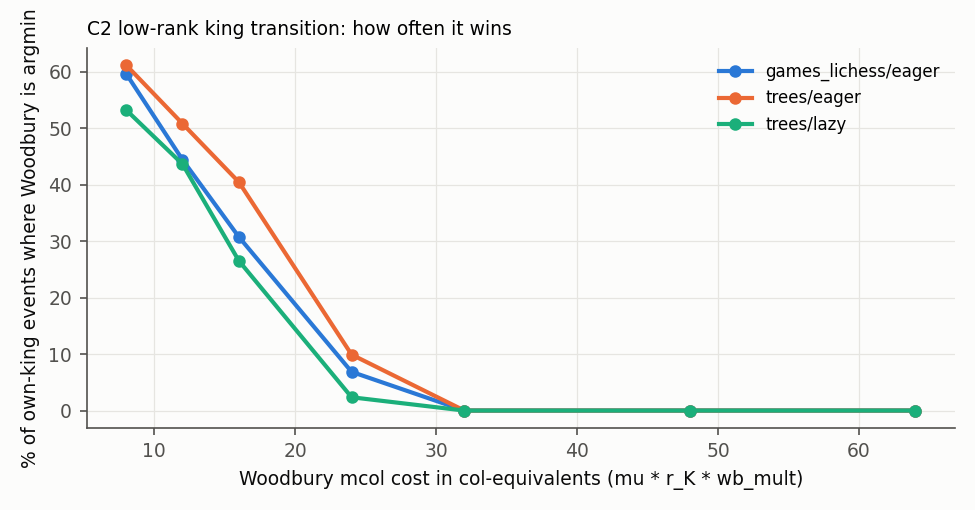
\includegraphics[width=0.75\linewidth]{figures/e4_woodbury_win_rate.png}
\caption{E4: Woodbury win rate at own-king events against its mcol cost $\mu\,r_K\,\mathrm{wb\_mult}$ in column equivalents.}\label{fig:e4}
\end{figure}

\paragraph{Results.}
Table~\ref{tab:e4} and Figure~\ref{fig:e4} show the results.
Woodbury is the argmin at own-king events only when $\mu r_K\,\mathrm{wb\_mult}\le24$ column-equivalents.
At the specification default ($r_K=16$, $\Delta U$ formed on the fly) it won 0\% of own-king events for every $\mu\in\{1,1.5,2\}$ on every swept dataset (Lichess games, eager and lazy trees; self-play was not swept).
This is consistent with hypothesis H2.
With precomputed $\Delta U$ at $\mu=1$ it wins 30.7\% of own-king events on Lichess games and uses 12.7\% fewer plain columns, but it adds 129,056 mcols, so the col-equivalent ratio is 0.9722 and FT bytes fall only 1.7\% (ratio 0.9828; 21,005.8 vs 21,372.8\,B per evaluation).
That also requires about 91 extra $y$-maintenance lanes per make event and a precomputed $\Delta U$ table (about 18.5\,MB, Section~\ref{sec:arch}).
On search trees Woodbury lowers column count slightly (0.9749 at $r_K=4$, $\mu=1$, eager) but increases FT bytes (ratio 1.0250 eager, 1.0596 lazy) once its mcols are counted (RESULTS.md \S2.5).
The cache-reset rerun gives the same picture: 0.9784 of VN's FT bytes on Lichess games at $r_K=16$ with precomputed $\Delta U$, and 1.0420 on eager trees (RESULTS.md \S2.7).

\subsection{E5: cost of the low-rank integer factorization}\label{sec:e5}

We used a synthetic planted table: one block, 32 buckets, 704 features and 256 lanes, with $W_k=W^0+U_kV$ (true rank 8) plus Gaussian noise, and an unstructured control.
$V_K$ is the top-$r_K$ right singular subspace of the stacked residuals.
In ``int factors'', $V_K$ is quantized to int8 and $U$ to int16 so that $UV_K$ is in table units at scale 64, and the integer product is materialized (the C2 exactness requirement).

\begin{table}[htbp]
\centering\small
\caption{E5: relative squared Frobenius error of the per-bucket residual (selected $r_K$; full table in \texttt{RESULTS.md}).}\label{tab:e5}
\begin{tabular}{@{}lrrrr@{}}
\toprule
table & $r_K$ & float SVD & \hd{int factors\\(materialized)} & \hd{plain int16\\table}\\
\midrule
planted\_rank8\_noise0.1 & 4 & 0.466 & 0.57 & 2.08e-05\\
 & 8 & 0.00978 & 0.218 & 2.08e-05\\
 & 16 & 0.0096 & 0.18 & 2.08e-05\\
 & 64 & 0.00856 & 0.164 & 2.08e-05\\
planted\_rank8\_noise0.5 & 8 & 0.195 & 0.315 & 1.65e-05\\
 & 16 & 0.191 & 0.315 & 1.65e-05\\
unstructured & 8 & 0.981 & 1 & 2.1e-05\\
 & 16 & 0.963 & 1 & 2.1e-05\\
 & 64 & 0.86 & 1 & 2.1e-05\\
\bottomrule
\end{tabular}
\end{table}

\begin{figure}[htbp]
\centering
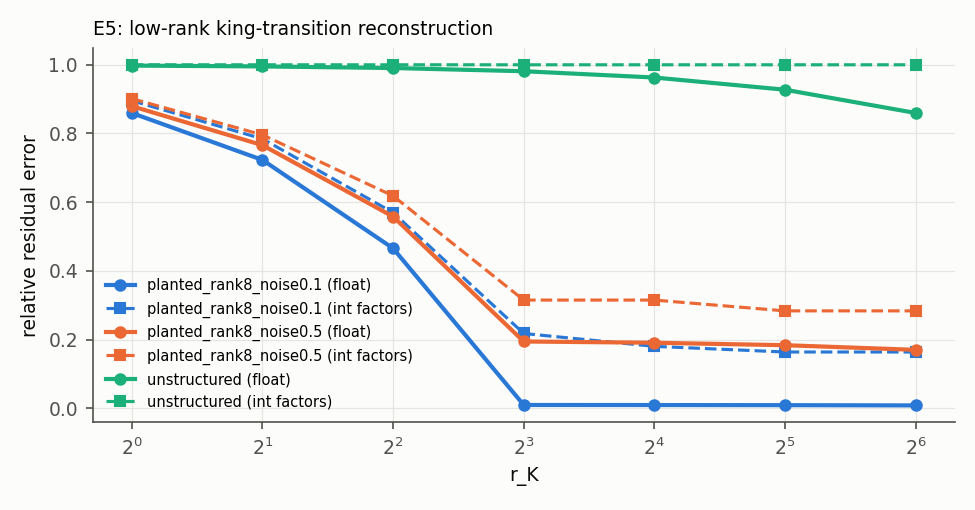
\includegraphics[width=0.8\linewidth]{figures/e5_rank.png}
\caption{E5: low-rank reconstruction error against $r_K$, float vs integer factors.}\label{fig:e5}
\end{figure}

\paragraph{Results.}
Table~\ref{tab:e5} and Figure~\ref{fig:e5} show the results.
On the planted rank-8 table, rank 8 recovers the residual in float (relative error 0.00978).
Rounding $U$ and $V_K$ so that their product is exact raises the error to 0.218, against 2.08e-05 for a plain int16 table at the same scale.
Without QAT, the integer-factor constraint is expensive.
On an unstructured table low rank does not help at all.
This experiment complements \texttt{lowrank\_proper} (T23).

\subsection{E6--E8: small training sanity checks}\label{sec:training}

\paragraph{Configuration.}
All models were trained for 6 epochs with batch size 1024 and Adam with a one-cycle schedule (max\_lr 2e-3), on seeds 0, 1, 2.
They use a single White-absolute perspective, no king buckets and no layer stacks.
The 175,984 Lichess positions (ply $\ge8$) were split by game into 140,307 training and 35,677 validation positions.
The synthetic teachers are $y=z(\mathrm{PST}\cdot\beta)+z(\text{pair term})+\text{noise}$, standardized to unit variance.
The pair term is (i) a low-rank $Q$ (rank 8, dense), (ii) a sparse ``attack-geometry'' $Q$ with 72,590 nonzero pairs, or (iii) both.
The models are listed below.
\begin{itemize}[leftmargin=*,itemsep=1pt]
\item M0\_L256 (201,281 parameters, 256 update lanes per changed feature).
\item M0s\_L192 (150,977 parameters, 192 lanes).
\item M1\_L192\_PSI\_r32\_m16 (176,593 parameters, 256 lanes). This model is matched to M0\_L256 in update lanes, not in bytes ($P2$ lanes are int32: $192\cdot2+32\cdot2+32\cdot4=576$\,B against 512\,B per changed feature) and not in readout MACs, which M0 does not pay.
\item M2\_L192\_explicit\_pairs (14,088,449 parameters). It also updates $L$ lanes for each changed active pair, of which there are on average 40.044 per position. M2 is a non-cost-matched reference with oracle knowledge of teacher (ii)'s support, run with 1 seed.
\end{itemize}

\begin{table}[htbp]
\centering\small
\caption{E6: held-out MSE (mean $\pm$ sample s.d.\ over 3 seeds; M2 one seed).}\label{tab:e6}
\begin{tabular}{@{}lrrrr@{}}
\toprule
teacher & M0\_L256 & M0s\_L192 & M1 (PSI) & M2 (explicit pairs)\\
\midrule
i\_lowrank & 0.0666 $\pm$ 0.0025 & 0.0706 $\pm$ 0.0022 & \textbf{0.0389} $\pm$ 0.0031 & 0.1476\\
ii\_sparse\_attack & 0.1607 $\pm$ 0.0003 & 0.1691 $\pm$ 0.0015 & 0.1487 $\pm$ 0.0035 & \textbf{0.0424}\\
iii\_both & 0.1612 $\pm$ 0.0022 & 0.1672 $\pm$ 0.0049 & 0.1336 $\pm$ 0.0020 & \textbf{0.1222}\\
\bottomrule
\end{tabular}
\end{table}

\begin{figure}[htbp]
\centering
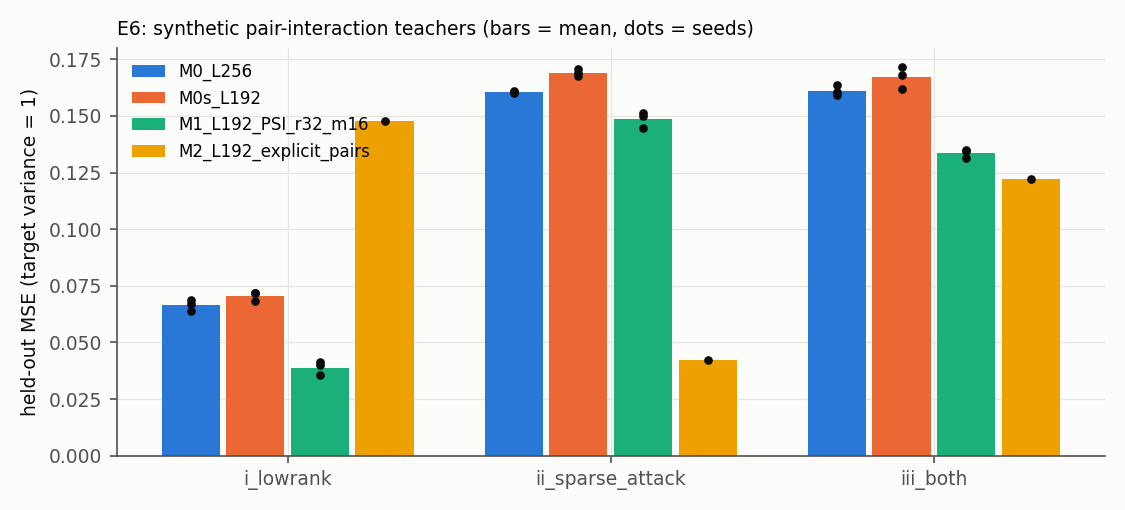
\includegraphics[width=0.8\linewidth]{figures/e6_training.png}
\caption{E6: held-out MSE per synthetic teacher and model.}\label{fig:e6}
\end{figure}

\paragraph{E6 results.}
Table~\ref{tab:e6} and Figure~\ref{fig:e6} show the results.
On all three synthetic pair teachers, the cost-matched M1 had lower held-out MSE than M0 and M0s.
The explicit-pair reference M2 is best on the sparse-attack teacher and on ``both'', and worst on the low-rank teacher; that last result is a single seed with a 14-million-parameter table and is likely undertrained, so it is not a meaningful comparison.
These teachers were \emph{built} to contain pair structure.
The result shows that PSI can learn such structure and nothing about chess evaluation.

\paragraph{Quantized PSI readout.}
We took M1 trained on teacher (iii), seed 0, quantized $V$ and $\Lambda$ to int8, and evaluated it on 4,000 validation positions.
The maximum $|P1|$ was 571 (bound 4064) and the maximum $P2$ was 43,527 (bound 516,128).
$P1^2-P2$ was even everywhere, and the maximum $|z_{\mathrm{int}}|$ was 21,117,603, below $2^{31}$.
The integer pipeline equalled a float evaluation of the quantized weights, and quantization gave a relative RMS error of 0.0161 in $z$.

\begin{table}[htbp]
\centering\small
\caption{E7 (tying under colour flip) and E8 (real-ish labels): held-out MSE.}\label{tab:e78}
\begin{tabular}{@{}llrr@{}}
\toprule
\multicolumn{4}{@{}l}{\emph{E7: M1, tied vs untied $V$} (untied 176,593 params, tied 164,305)}\\
teacher & & untied & tied\\
\midrule
iii\_both & & 0.1337 $\pm$ 0.0020 & 0.1498 $\pm$ 0.0062\\
iii\_both\_colour\_symmetrised & & 0.1362 $\pm$ 0.0029 & 0.1209 $\pm$ 0.0013\\
\midrule
\multicolumn{4}{@{}l}{\emph{E8: real-ish labels}}\\
label & mean predictor & M0\_L256 / M0s\_L192 & M1 (PSI)\\
\midrule
game\_result\_white\_pov & 0.2412 & 0.2807 $\pm$ 0.0030 / 0.2809 $\pm$ 0.0037 & 0.2920 $\pm$ 0.0022\\
material\_pst\_eval\_tanh & 0.3025 & 0.0158 $\pm$ 0.0008 / 0.0155 $\pm$ 0.0015 & 0.0158 $\pm$ 0.0023\\
\bottomrule
\end{tabular}
\end{table}

\paragraph{E7 and E8 results.}
Table~\ref{tab:e78} shows the results.
E7 retrains the untied M1 separately; the 0.0001 difference from Table~\ref{tab:e6} (0.1337 vs 0.1336) is run-to-run nondeterminism.
Tying $V$ under the colour flip \emph{hurt} on a teacher that is not colour-symmetric and helped on a colour-symmetrized one.
T21 held exactly on the trained tied model: the maximum $|P1(\text{flipped})-P1[\text{perm}]|$ and $|P2(\text{flipped})-P2[\text{perm}]|$ were both $0.00$.
On game results, every model was \emph{worse} than predicting the training mean, so this data and label combination is too small and noisy to compare models on. PSI was the worst.
On a linear material+PST label all models tie, as expected, because PSI has nothing to add to a label that is linear in $\beta$.
\textbf{No real-label benefit of PSI was observed.}

\subsection{Wall-clock proxy}

Table~\ref{tab:bench} gives the timings.
They were taken with Python on a 138.4\,MB int16 table (single thread, median of 5).
Unbatched timings measure Python dispatch more than memory traffic.
In batched torch kernels, a PSI quiet-move update costs 0.066 of an NNUE quiet-move update (4 columns), against a byte ratio of $384/8192=0.047$.
None of these timings predicts engine nps.

\begin{table}[htbp]
\centering\small
\caption{Wall-clock microbenchmark (rough proxy only; not engine speed).}\label{tab:bench}
\begin{tabular}{@{}lr@{\qquad}lrr@{}}
\toprule
unbatched kernel & ns/event & batched kernel & ns/event & GB/s\\
\midrule
NNUE quiet move, both persp., 4 cols & 9,572 & NNUE quiet, 4 cols & 7,578 & 1.081\\
PSI quiet move $P1,P2$ & 5,360 & PSI quiet $P1,P2$ & 503.502 & 0.763\\
refresh, 32 cols, one persp. & 49,841 & refresh, 32 cols & 46,933 & 1.396\\
Woodbury $r_K=16$ + 2 cols, one persp. & 39,960 & & &\\
PSI readout, one persp., $m=16$ & 27,140 & & &\\
\bottomrule
\end{tabular}
\end{table}

\subsection{Limitations of the experiments}
\begin{itemize}[leftmargin=*,itemsep=1pt]
\item The K32H3 model is simplified: threat and pawn-pair columns are not in the accumulator (threat bytes come from a proxy and are only counted), and there are no PSQT outputs and no layer stacks.
\item Search traces come from a toy alpha-beta (depth 3 + quiescence, 2,500-node cap, 116 of 200 trees truncated), not from Stockfish. Catch-up lengths, king-move frequencies and cache warmth are proxies.
\item The Stockfish policy is modelled from the specification text. The backward catch-up fill after a Finny refresh is not modelled, and pass costs are a uniform $4L$ bytes.
\item In the main E2--E4 run the Finny cache persists across games and trees (Section~\ref{sec:e3}); the rerun with a per-root reset changes the SF/SFmin ratios substantially but not the qualitative conclusions.
\item E1 covers subsets of the data (Section~\ref{sec:e1}).

\item Training uses one perspective, no king buckets, 6 epochs on 140k positions and synthetic teachers. M2 used 1 seed. E5 uses post-training quantization of the factors, not QAT.
\item Wall clock comes from Python on a 4\,GB laptop.
\end{itemize}
